\documentclass[25pt, portrait]{tikzposter}
\usepackage{authblk}
\usepackage{tikz}
\usepackage{adjustbox}
\usepackage{textcomp}
\usepackage{multicol}
\usepackage{amsmath}
% \usepackage{amssymb}
\usetikzlibrary{shapes, arrows.meta}
\usetheme{Default}

\title{\parbox{.85\textwidth}{ \begin{center}
Femtosecond-laser induced dynamics of CO on Ru(0001):\end{center}
\begin{center}\LARGE New insights from a hot-electron, electronic friction model including surface motion                                                                                           \end{center}}}
\author[1,2]{\underline{Robert Scholz}}
\author[1]{Gereon Flo\ss{}}
\author[1]{Peter Saalfrank}
\author[3]{Gernot F\"uchsel}
\author[4]{Ivor Lon\v{c}ari\'c}
\author[4,5,6]{J. I.~Juaristi}
\affil[1]{Institut f\"ur Chemie, Universit\"at Potsdam, Karl-Liebknecht-Str. 24-25, D-14476 Potsdam, Germany}
\affil[2]{Fritz-Haber-Institut der Max-Planck-Gesellschaft, Faradayweg 4-6, D-14195 Berlin, Germany}
\affil[3]{Universiteit Leiden, Gorlaeus Laboratories, Einsteinweg 55, 2333 Leiden, The Netherlands}
\affil[4]{Centro de F\'{\i}sica de Materiales CFM/MPC (CSIC-UPV/EHU), Paseo Manuel de Lardizabal 5, 20018 Donostia-San Sebasti\'an, Spain}
\affil[5]{Departamento de F\'{\i}sica de Materiales,
Facultad de Qu\'{\i}micas, 
Universidad del Pa\'{i}s Vasco (UPV/EHU), Apartado 1072, 20080 San Sebasti\'an, Spain}
\affil[6]{Donostia International Physics Center DIPC, P. Manuel de Lardizabal 4, 20018 San Sebasti\'an, Spain}

\makeatletter
\def\maketitle{\AB@maketitle}
\makeatother
\renewcommand{\Authfont}{\Large}
\renewcommand{\Affilfont}{\normalsize}

\settitle{ \centering \vbox{
\@titlegraphic \\[\TP@titlegraphictotitledistance] \centering
\color{titlefgcolor} {\bfseries \huge \sc \@title \par}
\vspace*{1em}
{ \@author \par}
}}


\begin{document}
  \maketitle[width=0.9\textwidth]
  \begin{columns}
    \column{0.42}
      \block{Introduction}{
		\innerblock{Motivation}{
		  \begin{itemize}
			\item research on small molecules adsorbed to metals is important for:
			\begin{itemize}
			  \item catalytic applications 
			  \item fundamental understanding of bonding
			\end{itemize}
			\item femtosecond(fs)-lasers are a valuable tool for such research as they
			\begin{itemize}
			  \item allow for investigations on small timescales   
			  \item open up new processes compared to heating (femtochemistry)
			  \item may enable specific control over catalytic reactions (photocatalysis) 
			\end{itemize}
			\item specific motivation for system CO/Ru(0001)
			\begin{itemize}
			  \item experimentally well studied regarding fs-laser irradiation, e.g. \cite{funk:00, nilsson:13}
			  \item fulldimensional \textit{ab-initio} potential recently developed in our group\cite{fuechsel:14}
			  \item details of this indicate interpretation of experiment \cite{nilsson:13} may be wrong
			\end{itemize}
		  \end{itemize}
		}
		\vspace{.5cm}

		\innerblock{How does fs-laser-irradiation affect metal surfaces?}{
% 		  \innerblock{How fs-laser-irradiation affects metal surfaces}{
% 		  \innerblock{What happens upon FL-irradiation of metal surfaces?}{
		  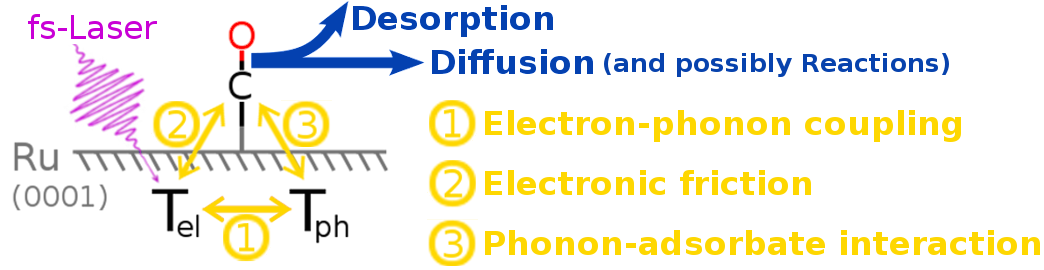
\includegraphics[width=.90\colwidth]{abb/modifiedSurfScheme.png}		    
		  \begin{minipage}[t]{.62\colwidth}
			\begin{itemize}
			  \item metals: 
			  %can be described as 
% 			    consist of an
					ion lattice plus quasi-free electron gas 
			  \item visible light is absorbed only by the electrons %only
			  \item produced electron-hole pairs thermalize quickly  
					$\Rightarrow$ ``hot'' Fermi-Dirac-distribution (after $\sim$10$\,$fs)
% 				  \item Fermi-Dirac schon hier?
						% \vbox syntax? (for the graphic)
			  \item electrons transfer part of energy to ion lattice, via \raisebox{-.18\baselineskip}{
\includegraphics[height=.8\baselineskip]{abb/one.png}}
			  \hspace{-0.5cm} \textbf{\color{innerblocktitlebgcolor!80!orange}electron-phonon coupling}\newline (phonons = lattice vibrations; quasi-particles)
			  \begin{itemize}
				\item electrons couple to phonons as their fast movement causes ``shockwaves'' in ion lattice
				\item equilibration process completes after $\sim$1$\,$ps			
			  \end{itemize}
			  \item[$\Rightarrow$] Thus, with fs-lasers, two different temperatures:
			  \begin{itemize}
				\item $T_\mathrm{el}$ - electron temperature
				\item $T_\mathrm{ph}$ - phonon temperature
% 					\item Two-Temperature Model (TTM)\cite{anisimov:74}
			  \end{itemize}
% 				  \item can be described with the Two-Temperature Model (TTM)
			\end{itemize}
		  \end{minipage}
		  \begin{adjustbox}{valign=t}
			\begin{minipage}[t]{.28\colwidth}
			  \begin{flushright}
				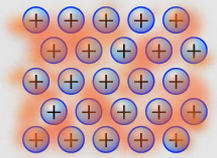
\includegraphics[width=.18\colwidth]{abb/elgas.png}$\,$\\[.6\baselineskip]
				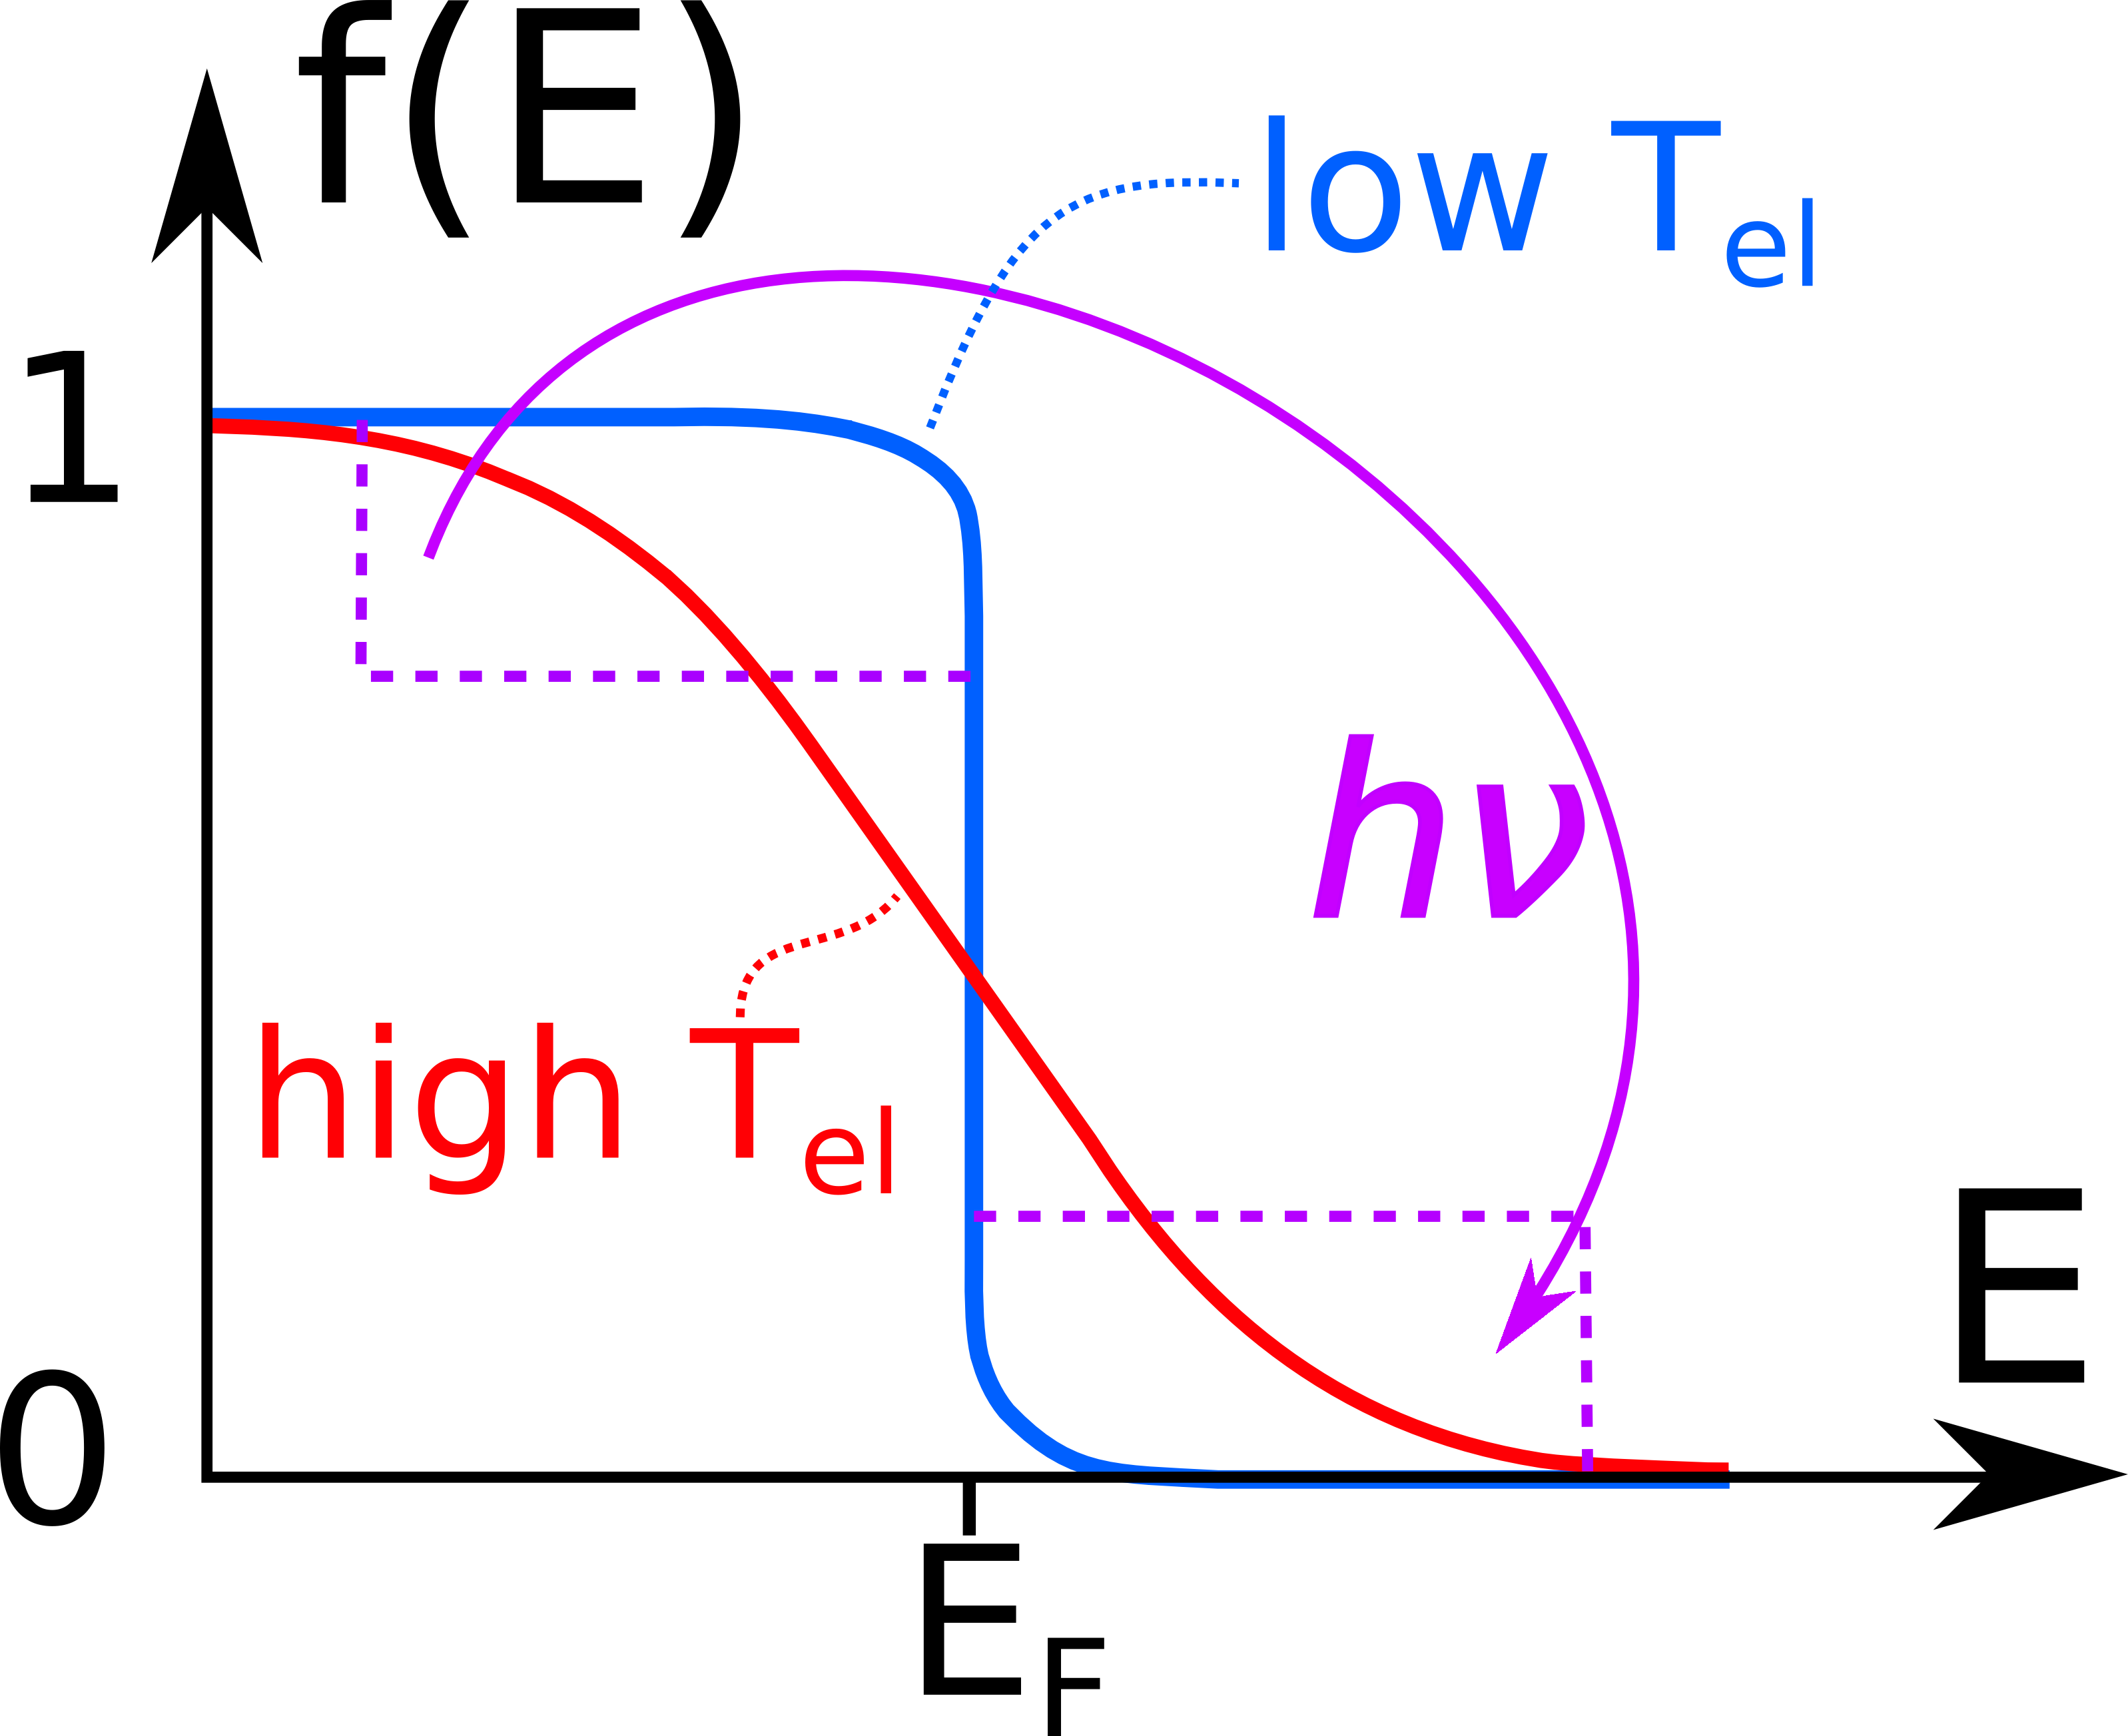
\includegraphics[width=.205\colwidth]{abb/fermi.png}\\[.3\baselineskip]
				\includegraphics[width=.26\colwidth]{abb/TTM_1pulse.eps}
			  \end{flushright}
			\end{minipage}
		  \end{adjustbox}
		  \begin{itemize}
			\item can be simulated using a Two-Temperature Model (2TM)%(TTM)
				  \cite{anisimov:74} (see right)
				  %consisting of two differential Equations 
		  \end{itemize}
		}
% 		  \includegraphics[width=.4\colwidth]{abb/TTM_1pulse.eps}
	  }
	\column{0.58}
	  \block{Models and Methods}{
		\innerblock{Six-dimensional Potential Energy Surface (6D PES)\cite{fuechsel:14}}{
		  \begin{minipage}[t]{.66\colwidth}
			\begin{itemize}
			  \item Basis for dynamics: precomputed PES from DFT (rPBE + D2) 
			\end{itemize}
			\begin{adjustbox}{valign=t}
			  \begin{minipage}[t]{.19\colwidth}
% 				  \vspace*{.5\baselineskip}
				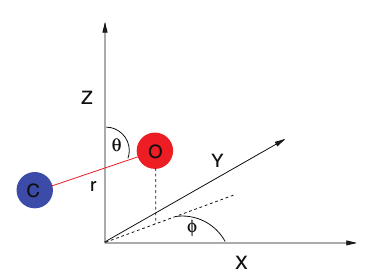
\includegraphics[width=.22\colwidth]{abb/6dimScheme.png}
			  \end{minipage}
			\end{adjustbox}
			\begin{minipage}[t]{.46\colwidth}
			  \begin{itemize}
				\item all 6 dimensions of the adsorbate
				\item analytical PES and gradients $\Rightarrow$ very fast % (once constructed)
				\item[$\Rightarrow$] number and length of trajectories can be large 
				\item downsides: -- surface atoms frozen $\Rightarrow$ no phonons 
				\newline \hspace*{4.5cm} -- had to be constructed first
			  \end{itemize}
			\end{minipage}
		  \end{minipage}
		  \begin{adjustbox}{valign=t}
			\begin{minipage}[t]{.35\colwidth}
			  \hspace*{-.01\colwidth}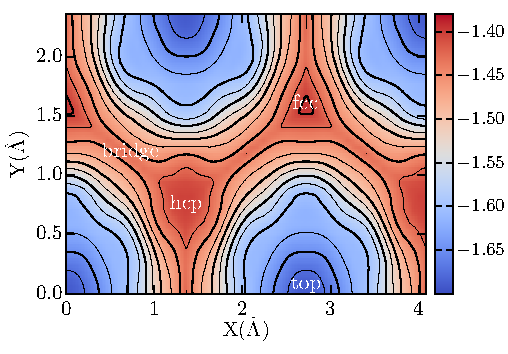
\includegraphics[width=.28\colwidth]{abb/fig_1b.pdf}
			\end{minipage}
		  \end{adjustbox}  
		}
		\vspace{.5cm}
	  
		\innerblock{Two-Temperature Model (2TM)\cite{anisimov:74}}{
		  \begin{minipage}[t]{.68\colwidth}
			\begin{itemize}
			  \item describes interaction of metal with laser, using two differential equations:
			\end{itemize}			  
			\begin{center}
			  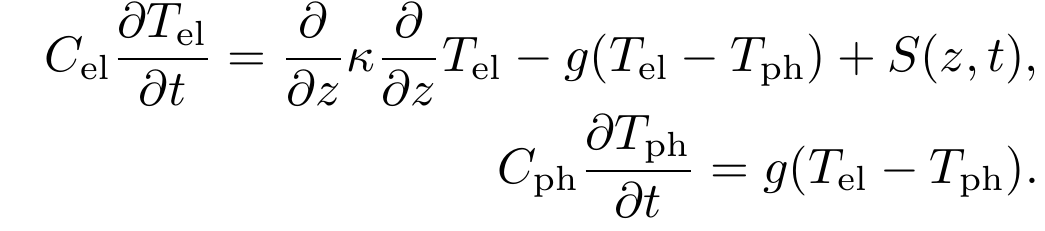
\includegraphics[width=.5\colwidth]{abb/2TM_equs.png}
			\end{center}
		  \end{minipage}
		  \begin{adjustbox}{valign=t}
			\begin{minipage}[t]{.25\colwidth}
			  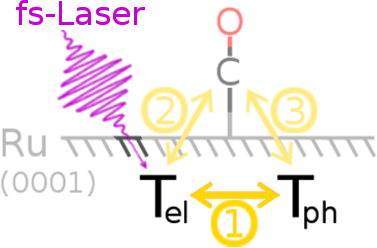
\includegraphics[width=.25\colwidth]{abb/Part1SurfScheme.png}
% 				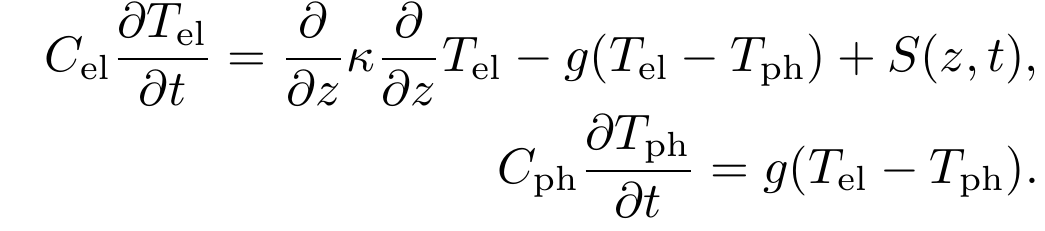
\includegraphics[width=.3\colwidth]{abb/2TM_equs.png}
			\end{minipage}
		  \end{adjustbox}
% 			\end{adjustbox}
		  \vspace{-1.2\baselineskip}
		  \begin{itemize}
			\item[$\Rightarrow$] get $T_\mathrm{el}$ and $T_\mathrm{ph}$ as $f(z,t)$ from laser parameters and material properties: 
			{\normalsize
			\begin{itemize}
			  \begin{minipage}[t]{.52\colwidth}
				\item laser wavelength $\lambda$ (affects penetretion depth into material)
				\item (effective) absorbed fluence $F$ (energy/area)
				\item pulse duration $\tau$ (all three appear in the ``source term'' $S(z, t)$)
			  \end{minipage}
			  \begin{minipage}[t]{.5\colwidth}
				\item electron and phonon heat capacities $C_\mathrm{el}$ and $C_\mathrm{ph}$
				\item electron heat conductivity $\kappa$ 			
				\item electron-phonon coupling constant $g$
			  \end{minipage}
			\end{itemize}				
			}
		  \end{itemize}	

		}
		\vspace{.5cm}
		  
		\innerblock{Electronic Friction: Langevin Dynamics\cite{headgordon:95} and Local~Density~Friction~Approximation~(LDFA)\cite{juaristi:08}}{
		  \begin{adjustbox}{valign=t}
			\begin{minipage}[t]{.26\colwidth}
			  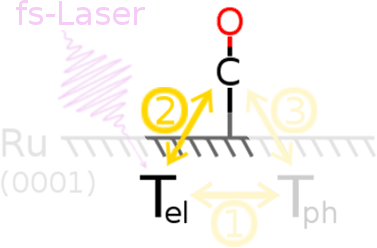
\includegraphics[width=.25\colwidth]{abb/Part2SurfScheme.png}
% 				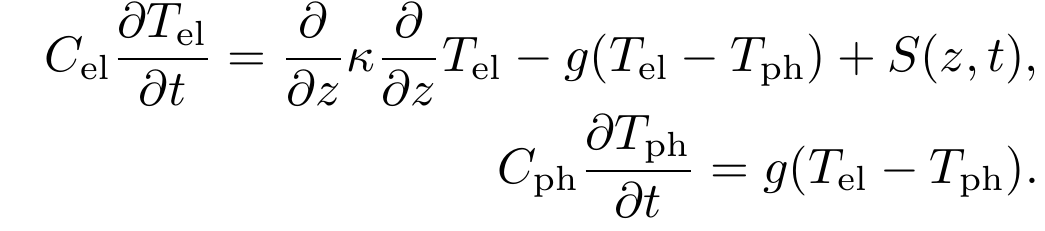
\includegraphics[width=.3\colwidth]{abb/2TM_equs.png}
			\end{minipage}
		  \end{adjustbox}
		  \begin{minipage}[t]{.6\colwidth}
			\begin{itemize}
			  \item Langevin equation of motion, a stochastical differential equation:%\\[-.9\baselineskip]
% 				\vspace{.2\baselineskip}
% 				\item describes interaction of  electron-hole-pairs with molecule
			\end{itemize}
			\vspace*{-.1\baselineskip}			  
			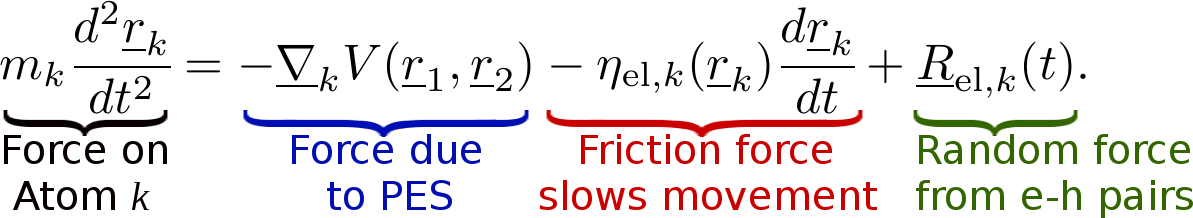
\includegraphics[width=.65\colwidth]{abb/Langevin_eq.png}
		  \end{minipage}
		  \vspace*{-.3\baselineskip}
		  \begin{itemize}
			\item describes movement of CO on the PES and interaction with electron-hole pairs (friction and excitation)
			\item Local Density Friction Approx. (LDFA): most simple model to calculate friction coefficients $\eta_{\mathrm{el},k}$
			\begin{itemize}
% 			    \item ``Local Density'' $\Rightarrow$ homogenous free electron gas (FEG)
			  \item Atom $k$ embedded in free electron gas with density of bare surface at current position $\underline{r}_k$
			\end{itemize}
			  \item Random forces $\underline{R}_{\mathrm{el},k}$: gaussian white noise,  dependent on both $\eta_{\mathrm{el},k}$ (from LDFA) and $T_\mathrm{el}$ (from 2TM)
			  \begin{itemize}
				\item justified by the 2. fluctuation dissipation theorem  \cite{kubo:66}, which relates friction and thermal movement 
			  \end{itemize}  
		  \end{itemize}

% 			\begin{adjustbox}{valign=t}
% 			  \begin{minipage}[t]{.5\colwidth}
% % 				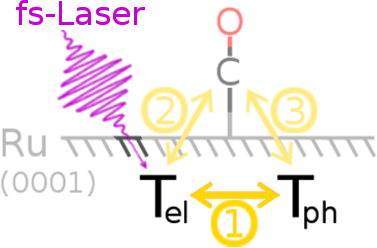
\includegraphics[width=.15\colwidth]{abb/Part1SurfScheme.png}\\[.3\baselineskip]
% 				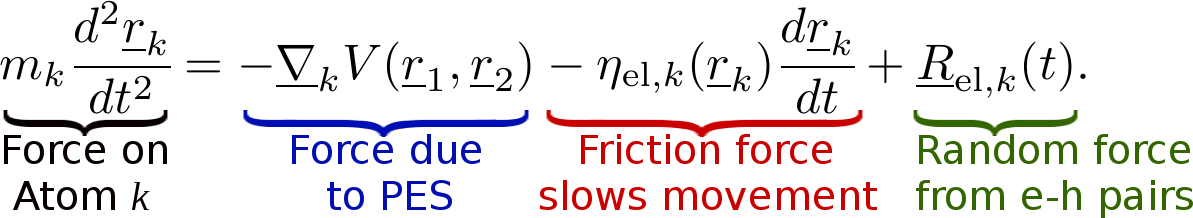
\includegraphics[width=.5\colwidth]{abb/Langevin_eq.png}
% 		      \end{minipage}
% 			\end{adjustbox}
		}
		\vspace{.5cm}
		
		\innerblock{Inclusion of Phonons: Generalized Langevin Oscillator(GLO)-model\cite{adelman:76, tully:80, busnengo:05}}{
		  \begin{adjustbox}{valign=t}
			\begin{minipage}[t]{.24\colwidth}
			  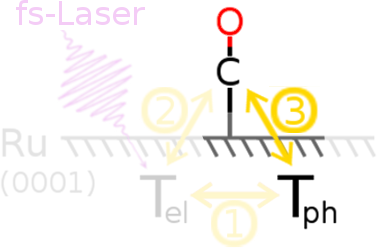
\includegraphics[width=.25\colwidth]{abb/Part3SurfScheme.png}
% 				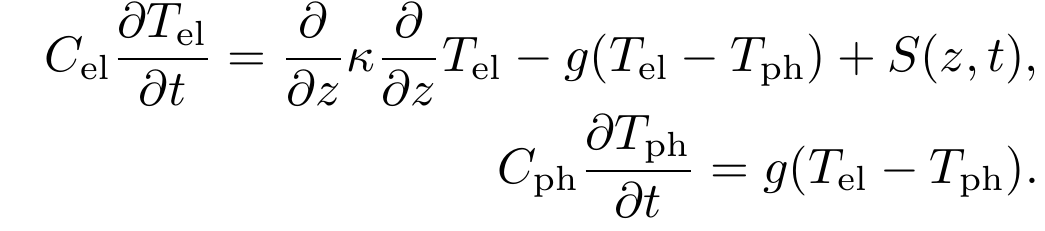
\includegraphics[width=.3\colwidth]{abb/2TM_equs.png}
			\end{minipage}
		  \end{adjustbox}
		  \begin{minipage}[t]{.7\colwidth}
			\begin{itemize}
			  \item influence of phonons modeled in an effective way (augments frozen surface)
			  \item entire surface understood as 3D oscillator (coordinates $\underline{r}_s$, mass $m_s = m_\mathrm{Ru}$)
			  \item coupling to molecule via shifting: %of the PES:
			  $\; V_\mathrm{GLO}(\underline{r}_\mathrm{C},\underline{r}_\mathrm{O};\underline{r}_s)=V(\underline{r}_\mathrm{C}-\underline{r}_s,\underline{r}_\mathrm{O}-\underline{r}_s)$ 
			  \item additionally coupled to ghost oscillator $\underline{r}_g$ to model influence of the bulk 
			  \begin{itemize}
				\item ghost oscillator is subject to friction $\eta_\mathrm{ph}$ and random forces $R_\mathrm{ph}(T_\mathrm{ph})$
			  \end{itemize}
			\end{itemize}
% 			  {\Large
% 			  \begin{equation*}
% 			    V_\mathrm{GLO}(\underline{r}_\mathrm{C},\underline{r}_\mathrm{O};\underline{r}_s)=V(\underline{r}_\mathrm{C}-\underline{r}_s,\underline{r}_\mathrm{O}-\underline{r}_s) 
% 			  \end{equation*}
% 			  }
% 			  \vspace*{-.1\baselineskip}			  
% 			  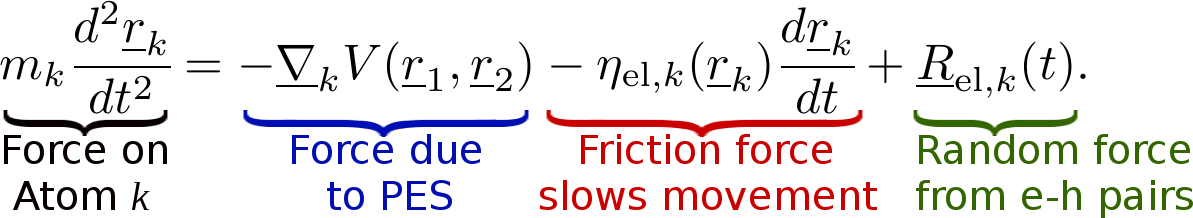
\includegraphics[width=.65\colwidth]{abb/Langevin_eq.png}
		  \end{minipage}
		}
	  }	
  \end{columns}
  \begin{columns}
  \column{.6}
  \block[titleoffsety=3cm,bodyoffsety=3cm,titleoffsetx=-.28\colwidth,titlewidthscale=.45,]{Results}{
	~\\[\baselineskip]
	
	~\\
	
  }
  \end{columns}
      %   \bibliography{/perm/scholz/phd/lit/biblio}
  \block{}{
    \begin{multicols}{2}
      \begin{thebibliography}{X}\normalsize
		
		\bibitem{funk:00}
% 		S. Funk, M. Bonn, D. N. Denzler, C. Hess et al., 
		S. Funk, M. Bonn, D. N. Denzler, C. Hess, M. Wolf and G. Ertl, 
		\emph{J. Chem. Phys.} \textbf{112}, 9888 (2000).
		
		\bibitem{nilsson:13}
% 		  M. Dell'Angela, T. Anniyev, M. Beye et al., 
		  M. Dell'Angela, T. Anniyev, M. Beye, R. Coffee, A. F\"ohlisch et al., 
		  \emph{Science} \textbf{339}, 1302 (2013).		  
		
		\bibitem{fuechsel:14}
		  G. F�chsel, J. C. Tremblay, and P. Saalfrank, 
		  \emph{J. Chem. Phys.} \textbf{141}, 094704 (2014).
		
		\bibitem{anisimov:74}
		  S. I. Anisimov, B. L. Kapeliovich, and T. L. Perel'man,
		  \emph{Sov. Phys.-JETP} \textbf{39}, 375 (1974).
		  
		\bibitem{headgordon:95}  
		M. Head-Gordon and J. C. Tully, \emph{J. Chem. Phys.} \textbf{103}, 10137 (1995).
		
		\bibitem{juaristi:08}
% 		J. I. Juaristi, M. Alducin, R. D�ez Mui�o, et al., 
		J. I. Juaristi, M. Alducin, R. D�ez Mui�o, H. F. Busnengo and A. Salin, 
		\emph{Phys. Rev. Lett.} \textbf{100}, 116102 (2008).
		
		\bibitem{adelman:76}
		S. A. Adelman and J. D. Doll, \emph{J. Chem. Phys.} \textbf{64}, 2375 (1976).
		
		\bibitem{tully:80}
		J. C. Tully, \emph{J. Chem. Phys.} \textbf{73}, 1975 (1980).
		
		\bibitem{busnengo:05}
		H. F. Busnengo, M. A. Di C�sare, W. Dong, and A. Salin,
		\emph{Phys. Rev. B} \textbf{72}, 125411 (2005).
		
		\bibitem{kubo:66}
		R. Kubo, \emph{Rep. Prog. Phys.} \textbf{29}, 255 (1966).
		
      \end{thebibliography}  
    \end{multicols}
  }
\end{document}


% \makeatletter
% \renewenvironment{tikzfigure}[1][]{
%   \def \rememberparameter{#1}
%   \vspace{10pt}
%   \refstepcounter{figurecounter}
%   \begin{center}
%   }{
%     \ifx\rememberparameter\@empty
%     \else %nothing
%     \\[10pt]
%     {\large Fig.~\thefigurecounter: \rememberparameter}
%     \fi
%   \end{center}
% }
% \makeatother
